\chapter{TINJAUAN PUSTAKA}

% Ubah konten-konten berikut sesuai dengan isi dari tinjauan pustaka
\section{Hasil penelitian/perancangan terdahulu}

\subsection{\emph{Ether Wallet} Menggunakan Ethereum Berbasis \emph{Multi Signature} }

Penulis pada \parencite{IdaBagus} menggunakan \emph{multisignature wallet} dengan harapan untuk menghindari kasus penipuan perseorangan yang memiliki wallet digital khususnya dengan teknik \emph{social engineering} seperti \emph{phising}, kemudian dapat bermanfaat dalam meningkatkan keamanan serta kepercayaan untuk lingkup kerjasama seperti diperusahaan karena untuk mengakses dompet membutuhkan konfirmasi dari kedua belah pihak. \emph{Multi Signature Wallet} sendiri merupakan dompet yang dapat dijalankan ketika telah mendapatkan persetujuan dari alamat dompet lainnya yang dimiliki oleh pengguna. 

% Contoh input gambar dengan format *.jpg
\begin{figure} [ht] \centering
  % Nama dari file gambar yang diinputkan
  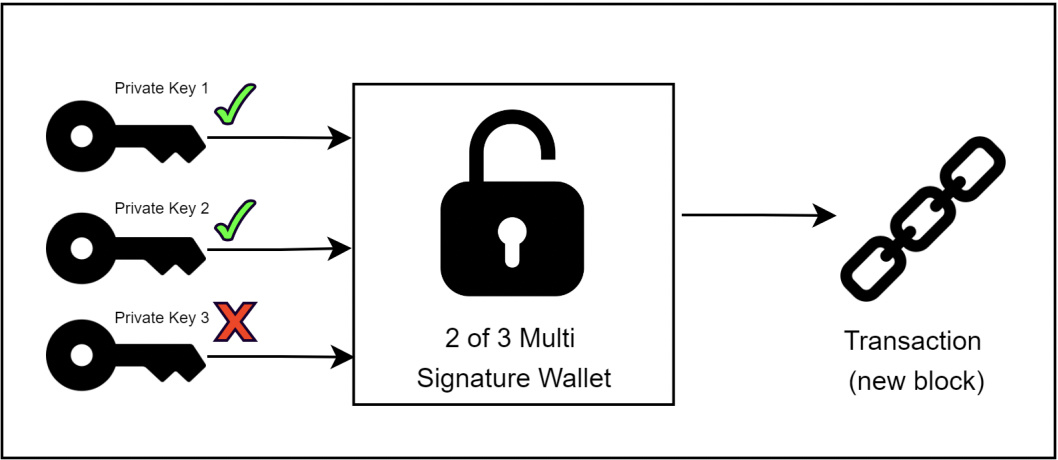
\includegraphics[scale=0.6]{gambar/img-multisignature-wallet.png}
  % Keterangan gambar yang diinputkan
  \caption{Multi Sig Wallet Konfirmasi 2 Akun}
  % Label referensi dari gambar yang diinputkan
  \label{fig:Multisignature Wallet}
\end{figure}

Walaupun begitu, dalam kasus penggunaan \emph{shared ownership}, \emph{multisignature wallet} memiliki berbagai kekurangan dalam praktiknya. Jika dibandingkan dengan pembagian kepemilikan dalam kasus suatu pembelian saham perusahaan, pembeli saham tidak perlu berhubungan langsung dengan pemilik-pemilik lainnya. Akan tetapi penggunaan \emph{multisignature wallet} ini seorang pembeli saham tersebut harus berkomunikasi dengan pemilik lain untuk menambahkan \emph{private key} yang tentunya hal ini lah yang cukup menyulitkan bagi calon pembeli saham baru tersebut. 

\section{Teori/Konsep Dasar}

\subsection{Blockchain}

% Contoh input gambar dengan format *.jpg
\begin{figure} [ht] \centering
  % Nama dari file gambar yang diinputkan
  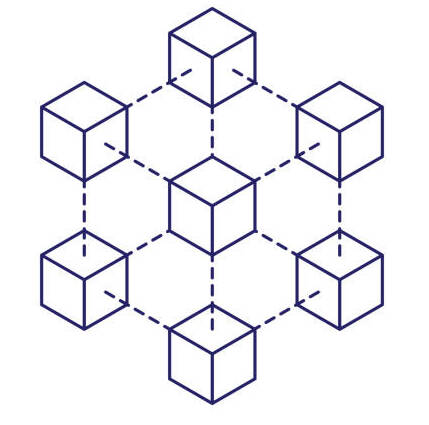
\includegraphics[scale=1.2]{gambar/img-blockchain-illustration.jpg}
  % Keterangan gambar yang diinputkan
  \caption{Ilustrasi \emph{Blockchain}}
  % Label referensi dari gambar yang diinputkan
  \label{fig:Metaverse}
\end{figure}

% Contoh penggunaan referensi dari pustaka
\emph{Blockchain} adalah \emph{ledger} atau buku besar terdistribusi yang dibagikan diantara node-node dalam jaringan komputer \parencite{LouiseAxon}. Ledger atau buku besar ini didistribusikan antar \emph{node}-\emph{node} dalam \emph{Blockchain} secara \emph{peer-to-peer} dengan teknik kriptografi. Data-data yang berada di dalam \emph{Blockchain} tidak dapat diubah hanya dapat ditambahkan. 

\emph{Blockchain} juga merupakan suatu \emph{Database}. Walaupun begitu, \emph{Blockchain} memiliki perbedaan yaitu data-data pada \emph{Blockchain} tidak disimpan oleh pihak tinggal melainkan didistribusikan antar \emph{node}-\emph{node}. Selain itu perbedaan \emph{Blockchain} dengan \emph{Database} umumnya adalah bagaimana data di dalam \emph{Blockchain} dibentuk. Sebuah \emph{Blockchain} menyimpan berbagai informasi bersama dalam suatu kelompok yang dinamakan \emph{Block}. \emph{Block} memiliki penyimpanannya sendiri, dimana ketika kapasitas penyimpanannya terpenuhi maka \emph{Block} tersebut akan tertutup dan dihubungkan dengan blok sebelumnya.
Hal tersebut berbeda dengan \emph{Database} yang umumnya menyimpan data-data dalam suatu table. Setiap \emph{Block} properti khusus selain data yang disimpan seperti contohnya adalah \emph{timestamp} yang menandakan kapan \emph{Block} tersebut dibuat.

Data di dalam \emph{Blockchain} bersifat \emph{immutable} yang berarti bahwa sekali data ditambahkan kedalam \emph{Blockchain}, hampir tidak mungkin
untuk mengubah data itu dan data sebelumnya pun praktis tidak berubah. Dengan kata
lain, blok yang ditambahkan ke Blockchain tidak dapat diubah, yang memungkinkan Blockchain menjadi buku besar transaksi yang tidak dapat dirusak maupun diubah. Namun,
hal itu dapat saja berbeda, bahwa Blockhain dapat diubah dalam skenario langka di mana
kerjasama mengubah jaringan Blockchain oleh peretas berhasil mendapatkan lebih dari
51 persen kekuatan jaringan dalam waktu yang relatif singkat. Hal ini lah yang menjadikan \emph{Blockchain} lebih aman dari model penyimpanan data pada umumnya. 

Di dalam \emph{Blockchain} tidak ada pihak sentral yang memiliki otoritas lebih tinggi dari yang lain sehingga jika terjadi perubahan bagaimana \emph{Blockchain} bekerja ditentukan oleh kesepakatan \emph{node}-\emph{node} di dalam \emph{Blockchain} tersebut. Kesepakatan ini juga sering dikenal dengan istilah konsensus dan tiap \emph{Blockchain} memiliki konsensusnya masing-masing.
Konsensu menjadi hal yang paling penting untuk mengubah sistem dari suatu \emph{Blockchain}, sehingga
Blockchain ini juga digambarkan seperangkat aturan konsensus, yang mengatur transaksi
mulai dari transaksi apa yang dilakukan hingga apa yang membuat transaksi tersebut
kemudian dapat divalidasi, inilah yang membuatnya menjadi terdesentralisasi. \emph{Blockchain}
dapat dikatakan sebuah mesin yang memproses aturan sesuai dengan konsensus tersusun
dari rantai blok yang diamankan secara kriptografis. Konsensus pada \emph{Blockchain} ini bersifat memaksa terhadap penambang untuk mengikuti dan bekerjasama dalam penegakan
aturannya. \parencite{antonopoulos2018mastering}

Secara ringkas \emph{Blockchain} memiliki berbagai keunggulan diantaranya adalah sebagai berikut
\begin{itemize}
    \item \emph{Transparant}, dalam \emph{blockchain} menerapkan sistem yang transparan sehingga dapat dilihat oleh berbagai orang.
    \item \emph{Immutability}, data yang dibuat didalam \emph{blockchain} tidak dapat ubah setelah dibuat.
    \item \emph{Secure}, dengan adanya implementasi kriptografi seperti validasi dengan fungsi hash membuat data yang ada pada Blockchain lebih aman.
    \item \emph{Traceability}, pada setiap blok dalam \emph{blockchain} menyimpan hash dari blok sebelumnya sehingga data pada Blockchain dapat dilacak dengan mudah.
    \item \emph{Anonymous}, setiap transaksi yang dibuat dapat dilihat oleh orang lain akan tetapi identitasnya tidak dapat diketahui dikarenakan yang ditampilkan adalah alamat \emph{wallet} atau yang merupakan \emph{public key}.
  \end{itemize}

\subsection{\emph{Node}}

\emph{Node} di dalam \emph{Blockchain} memiliki tanggung jawab untuk bertindak sebagai titik komunikasi yang dapat membuat, menerima, mengirim, dan mengyimpan data di dalam jaringan \emph{Blockchain}. Node pada dasarnya merupakan komputer yang berisi salinan dari riwayat transaksi dan data \emph{Blockchain}. \emph{Node} memiliki jenis dan fungsinya masing-masing. \parentext{DouglasTjokrostetio}

\subsubsection{\emph{Node} Penuh (\emph{Full Node})}

\emph{Node} penuh merupakan \emph{Node} yang berperan vital dalam \emph{Blockchain} dikarenakn bertindak sebagai \emph{fully validating node} atau \emph{Node} yang sepenuhnya melakukan validasi setiap transaksi yang dilakukan. \emph{Node} penuh pada awalnya akan mengunduh seluruh salinan \emph{Blockchain}. Untuk \emph{Bitcoin} sendiri pada tahun 2021 suatu \emph{Full Node} membutuhkan ruang penyimpanan 350 \emph{gigabyte} (GB) untuk mengunduh seluruh data \emph{Blockchain}.

\subsubsection{\emph{Node} Listening (\emph{Supernode})} dan Node Tersembunyi (Non-Listening Node)

\emph{Node Listeng} atau \emph{supernode} adalah \emph{Full Node} yang terlihat oleh publik. Ketika suatu \emph{Node} melakukan komunikasi dengan \emph{Node} listening, node ini akan mengomunikasikan dengan memberikan informasi ke \emph{Node} tersebut. Berbeda dengan \emph{Node listening} , \emph{Node non-listening} tidak terlihat oleh publik. \emph{Node} ini beroperasi di belakng \emph{firewall} atau dikonfigurasi supaya tidak mendengarkan komunikasi dari luar.

\subsubsection{\emph{Node Miner}}

Ekosistem \emph{Blockchain} yang menggunakan konsensus tertentu seperti \emph{proof-of-work} yang diterapkan oleh \emph{Bitcoin} membutuhkan \emph{Full Node} yang berperan sebagai \emph{Miner}. \emph{Node} ini berperan dalam menambahkan data transaksi ke \emph{Blockhain} dan akan menerima \emph{reward} seperti kripto.

\subsubsection{\emph{Lightweight Node}}

\emph{Node} ringan yang juga dikenal sebagai klien \emph{SPV} (\emph{Simplified Payment Verification}), adalah node yang menggunakan jaringan \emph{Blockchain} tapi tidak sepenuhnya bertindak layaknya \emph{Full Node}. Klien SPV tidak berkontribusi dalam keamanan suatu \emph{Blockchain} dikarenakan tidak menyimpan salinan \emph{Blockchain} dan melakukan proses validasi transaksi. Klien SPV hanya melakukan pemeriksaan apakah suatu informasi dapat ditermukan dalam jaringan \emph{Blockchain}.

\subsection{\emph{Block}}

% Contoh input gambar dengan format *.jpg
\begin{figure} [ht] \centering
  % Nama dari file gambar yang diinputkan
  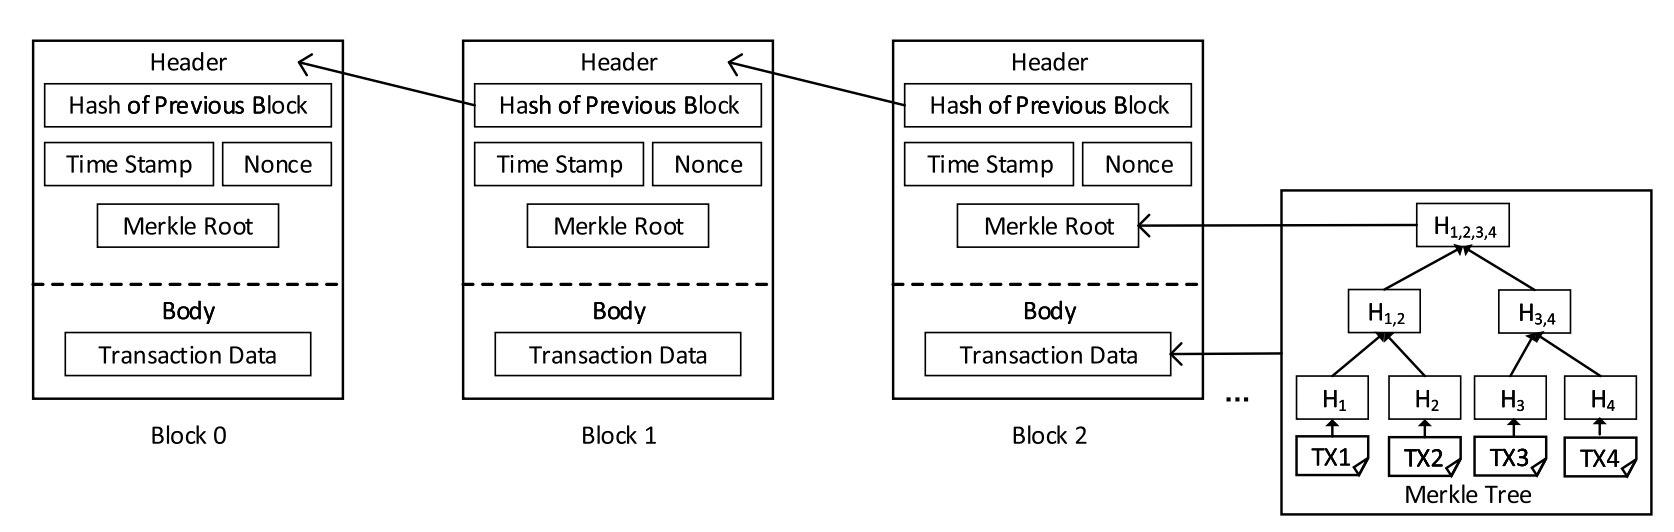
\includegraphics[scale=0.55]{gambar/img-block-structure.png}
  % Keterangan gambar yang diinputkan
  \caption{Struktur \emph{Block} pada \emph{Blockchain}}
  % Label referensi dari gambar yang diinputkan
  \label{fig:Metaverse}
\end{figure}

Di dalam jaringan \emph{Blockchain} suatu transaksi yang telah divalidasi oleh \emph{Node} akan disimpan ke dalam \emph{Block}. \emph{Block} sendiri tersusun dari \emph{Header} dan \emph{Body}. \emph{Header Block} tersusun dari \emph{Hash} dari \emph{Block} sebelumnya, \emph{timestamp}, \emph{Nonce}, dan \emph{Merkle Tree}. Nilai dari \emph{hash} diperoleh dari \emph{Header Block} sebelumnya yang telah dilakukan \emph{Hashing}. Memasukan \emph{Header Block} sebelumnya ke \emph{Block} saat ini membuat \emph{Block}-\emph{Block} dalam \emph{Blockchain} sehingga menciptakan suatu ikatan (\emph{chain}) dan terntunya menjadikannya saling terhubung antar satu \emph{Block} dengan \emph{Block} lainnya. Hal ini pun yang membuat \emph{Blockchain} aman dikarenakan jika akan melakukan pengubahan pada satu \emph{Block} maka seluruh \emph{Block} juga perlu diubah jika tidak akan dapat divalidasi melalui nilai \emph{Hash}-nya. \emph{Timestamp} sendiri berisi informasi kapan waktu \emph{Block} tersebut dibuat. \emph{Nonce} (number only used once) adalah angka yang dipecahakn oleh \emph{miner}. Angka ini diubah oleh \emph{miner} untuk memperoleh \emph{Merkle tree root hash} yang berdada di bawah nilai target. \emph{Merkle tree root hash} sendiri merupakan suatu data yang meringkas seluruh transaksi dalam \emph{Block} tersebut dan digunakan untuk memudahkan proses validasi. \emph{Body} pada suatu \emph{Block} sendiri berisi daftar transaksi yang disimpan.     
\parencite{LiangYiangBlockchainDynamicSpectrum}

\subsection{\emph{Wallet}}

\emph{Wallet} yang digunakan dalam transaksi pada \emph{Blockchain} merupakan suatu perangkat lunak yang memungkinkan antar pengguna untuk bertransaksi satu dengan yang lainnya dan merekam saldo dari pengguna. Berbeda dengan uang fiat, \emph{cryptocurrency} dalam \emph{Blockchain} tidak disimpan secara fisik. Di dalam \emph{Wallet} terdapat \emph{public key} dan \emph{private key}. Kedua \emph{Key} ini merupakan pasangan yang diperoleh dari algoritma asimetris dalam kriptografi. \emph{Public key} digunakan sebagai identifikasi dalam melakukan penerimaan atau pengiriman layaknya nomor rekening bank. Sedangkan \emph{Private key} digunakan untuk melakukan proses \emph{Authorization} dalam mengakses \emph{Wallet} tersebut. Selain itu juga terdapat \emph{address} dalam \emph{wallet} yang berfungsi sebagai pengenal unik yang digunakan untuk memfasilitasi proses pembayaran. \emph{Address} sendiri lebih singkat dibandingkan \emph{Public key} dikarenakan diperoleh dari melakukan \emph{hash} terhadap \emph{Public key}. 
\parencite{JokicStevo}

Terdapat dua jenis utama \emph{Wallet} dalam \emph{Blockchain} yaitu \emph{hot wallet} dan \emph{cold storage}. \emph{Hot wallet} adalah \emph{wallet} kripto yang biasanya terkoneksi dengan internet. \emph{Hot wallet} tidak harus selalu terhubung dengan internet. Dengan melakukan pengunduhan data, pengguna dapat menyimpan informasi milik mereka di perangkat pribadi. Wallet jenis ini umumnya memiliki tingkat kerentanan yang tinggi. Di lain sisi \emph{Cold storage} adalah \emph{Wallet} yang tidak terhubung ke inernet.

\subsection{Ethereum}

Ethereum adalah salah contoh dari \emph{Blockchain} yang diciptakan setelah \emph{Bitcoin}. Namun \emph{Ethereum} lebih dari sekedar \emph{Bitcoin} yang mendistribusikan catatan, \emph{Ethereum} adalah jaringan mesin virtual terdistribusi sehingga selain memiliki kemampuan untuk menyimpan suatu catatan dan mendistribusikannya, \emph{Ethereum} juga memiliki kemampuan untuk mengeksekusi suatu program yang berada di dalamnya. Hal tersebut berkat adanya \emph{EVM (Ethereum Virtual Machine)} yang mampu mengeksekusi program yang berada dalam \emph{node-node} pada \emph{Blockchain} \emph{Ethereum} sehingga \emph{Blockchain} ini tidak hanya sebagai \emph{Blockchain} catatan berjalan tetapi juga sebagai mesin virtual berjalan. Program yang berjalan di atas \emph{EVM} dikenal juga sebagai \emph{Smart Contract} dimana suatu fungsi di dalam \emph{Smart Contract} akan dieksekusi ketika suatu kondisi tertentu terpenuhi. Dengan kemampuan mengeksekusi \emph{Smart Contract} \emph{Ethereum} menciptakan era baru pada perkembangan \emph{Blockchain} yang memungkinkan para pengembang dapat menjalankan aplikasi terdistribusi atau juga dikenal sebagai \emph{DApps}.  Jaringan komputer terdistribusi \emph{Ethereum} dengan mudah menyediakan keamanan, keandalan, dan daya komputasi yang
diperlukan untuk melaksanakan pengaturan yang dirancang. Blockchain Ethereum pun
juga dapat dicari secara publik (Jani, 2017)

Ethereum dikembangan pada tahun 2013 oleh Vitalik Buterin, seorang programmer yang memiliki minat pada perkembangan \emph{Blockchain} dan \emph{Bitcoin}.
Vitalik berpikir untuk memperluas kemampuan dari Bitcoin dan Mastercoin. Pada bulan Okteber di tahun tersebut, Vitalik mengusulkan pendekatan yang lebih umum kepada tim
Mastercoin, yang memungkinkan kontrak fleksibel dan dapat ditulis untuk menggantikan
bahasa kontrak khusus Mastercoin. Tim Mastercoin terkesan namun belum bisa menerima usulan dalam bentuk proposal tersebut karena masih terkesan ’kasaran’. Maka dari
itu, Vitalik yang juga salah satu pendiri Bitcoin Magazine, pada bulan Desember menerbitkan whitepaper yang mengusulkan implementasi Blockchain baru yang lebih fungsional.
Proposal baru ini kemudian dinamakan Blockhain Ethereum. Setelah mendapatkan minat
dan menarik teknis dan finansial dukungan, Yayasan Ethereum, sebuah organisasi nirlaba
Swiss, didirikan dan menjadi pengembang Ethereum. Proses pengembangan ini berlangsung sejak saat itu, hingga pada tanggal 30 Juli 2015, Ethereum blok pertama berhasil
di tambang (Antonopoulos Wood, 2018). Ethereum ini kemudian dinamakan Frontier.
serta saat bersamaan Wallet Ethereum versi beta juga dibentuk. Pengembangan sampai saat ini sudah ada 2 kali pembaharuan project Ethereum, yaitu Homestead ditahun
2016, dan Byzantium di tahun 2018 (Infante, 2019). Kemudian perubahan versi keempat,
direncanakan di release tahun ini dengan nama Theta.

\subsection{\emph{EVM (Ethereum Virtual Machine)}}

% Contoh input gambar dengan format *.jpg
\begin{figure} [ht] \centering
  % Nama dari file gambar yang diinputkan
  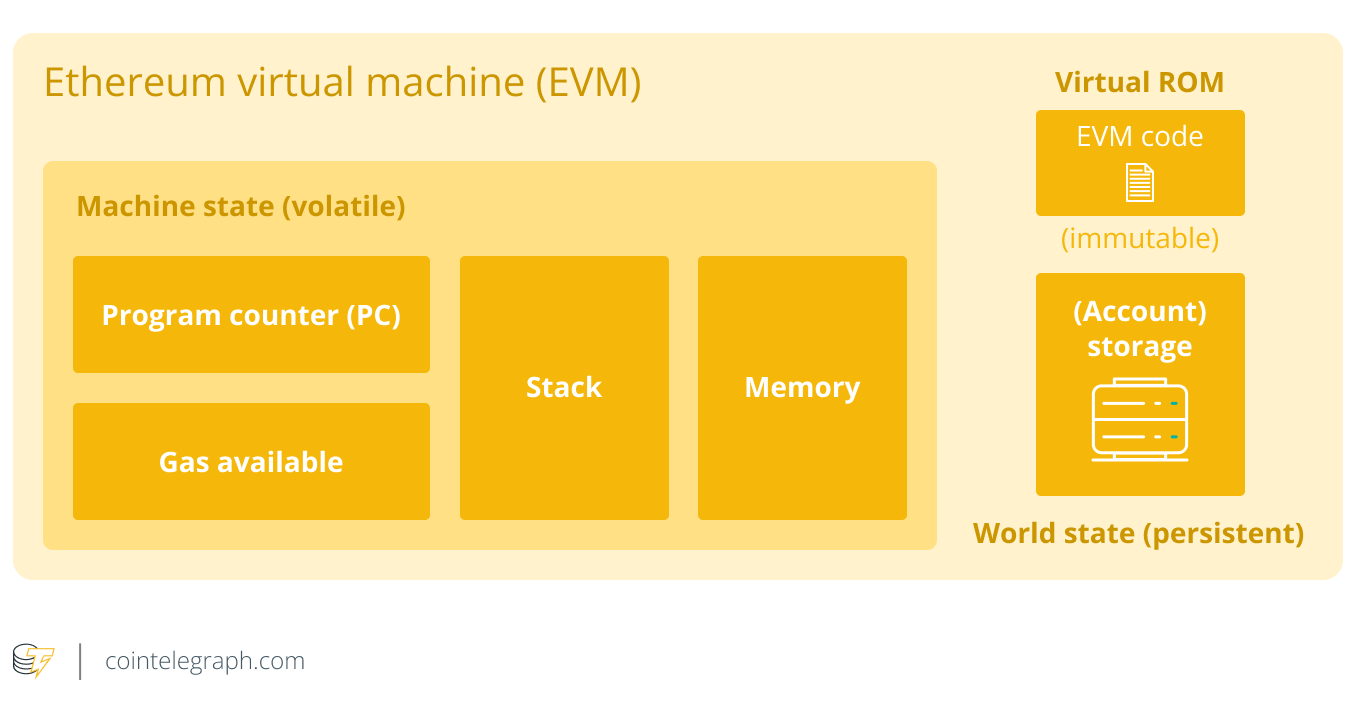
\includegraphics[scale=0.3]{gambar/img-evm.png}
  % Keterangan gambar yang diinputkan
  \caption{Ethereum Virtual Machine}
  % Label referensi dari gambar yang diinputkan
  \label{fig:Metaverse}
\end{figure}

\emph{EVM (Ethereum Virtual Machine)} adalah mesin komputasi virtual yang memiliki kemampuan untuk mengeksekusi suatu perintah atau fungsi pada \emph{Smart Contract}. \emph{EVM} terisolasi dari lingkungan di luarnya sehingga kode \emph{Smart Contract} yang berjalan di atasnya tidak memiliki kemampuan untuk mengakses jaringan, sistem berkas, atau proses lainnya. Ethereum sendiri memiliki dua jenis akun yaitu EOA (Externally-owned account) yang dikendalikan oleh siapapun yang memiliki \emph{private key} dan \emph{Contract account} yang dikendalikan oleh perintah-perintah yang berada di dalam \emph{Smart Contract}. Setiap \emph{Smart Contract} yang di \emph{deploy} pada jaringan \emph{Ethereum} memiliki alamat yang merupakan bagian dari \emph{Contract Account}. Kedua jenis akun hanya dapat berinteraksi dalam \emph{Smart Contract} yang dieksekusi oleh EVM.

\subsection{\emph{Ethereum Account}}

% Contoh input gambar dengan format *.jpg
\begin{figure} [ht] \centering
  % Nama dari file gambar yang diinputkan
  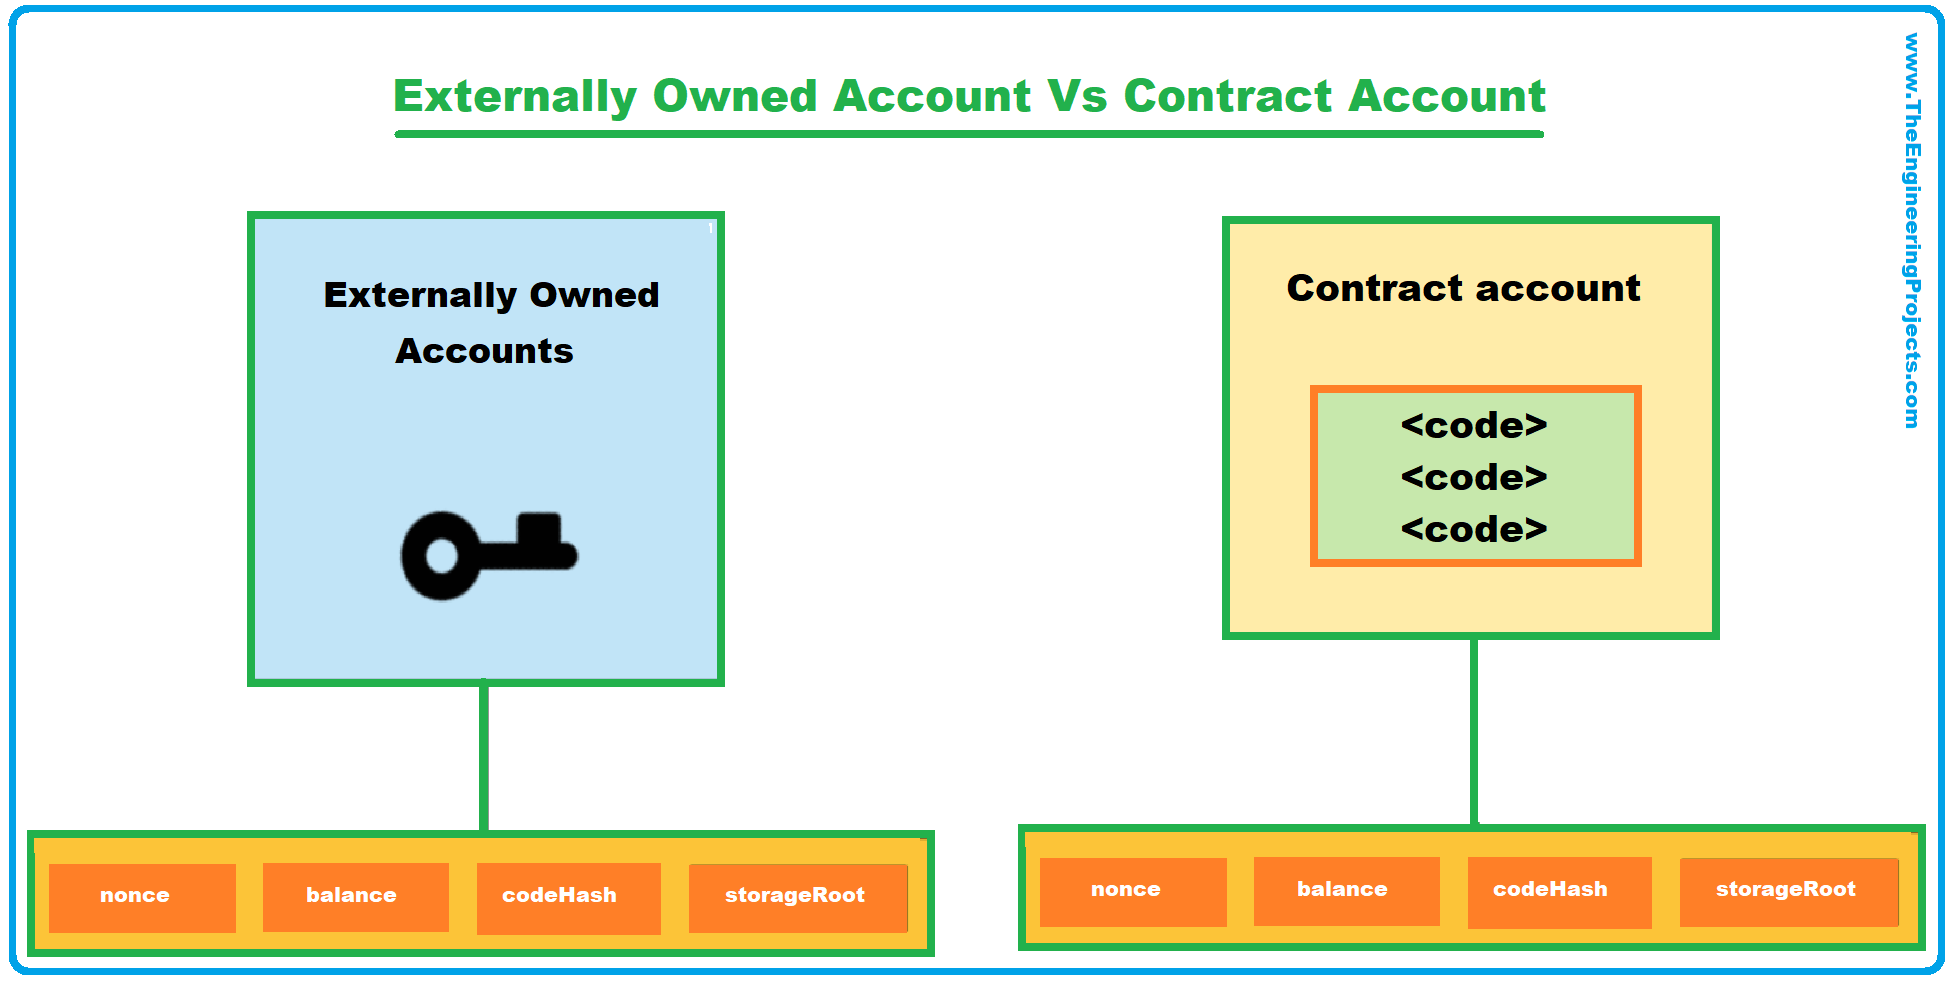
\includegraphics[scale=0.2]{gambar/img-ethereum-account.png}
  % Keterangan gambar yang diinputkan
  \caption{\emph{Account Ethereum}}
  % Label referensi dari gambar yang diinputkan
  \label{fig:Metaverse}
\end{figure}

Dalam melakukan transaksi dalam \emph{Blockchain Ethereum} pengguna memerlukan \emph{account}. \emph{Account} pada \emph{Blockchain Ethereum} sendiri terbagi menjadi dua jenis yaitu EOA (Externally Owned Account) dan \emph{Contract Account}. EOA adalah akun yang dikendalikan dan dimiliki masing-masing individu. Jenis akun ini dapat mengirim transaksi ke sesama \emph{EOA} ataupun akun kontrak. Akun ini memiliki \emph{Public key} dan \emph{Private key} yang terkait. Selain itu juga memiliki \emph{address} yang dihasilkan dari \emph{Public key} yang dimiliki. Ketika EOA dibuat, \emph{Private key} dienkripsi dengan kata sandi yang diberikan dalam pembuatan akun. Untuk mengakses dan melakukan transaksi pada EOA, \emph{Private key} dan kata sandi akan diperlukan. Akun kontrak sendiri dihasilkan dari proses \emph{deployment smart contract} oleh \emph{EOA} dan dikendalikan oleh kode-kode di dalamnya dalam melakukan transaksi. Kode-kode di dalam akun kontrak dieksekusi ketika dipanggil oleh EOA ataupun kontrak lain.  
\parencite{BahgaArshdeep}

\subsection{\emph{Transaction}}

% Contoh input gambar dengan format *.jpg
\begin{figure} [ht] \centering
  % Nama dari file gambar yang diinputkan
  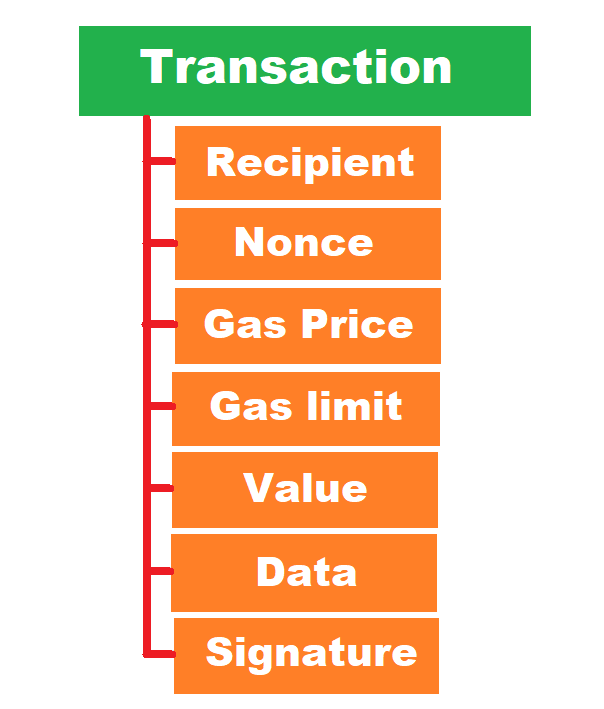
\includegraphics[scale=0.4]{gambar/img-transaction-structure.png}
  % Keterangan gambar yang diinputkan
  \caption{Struktur Transaksi}
  % Label referensi dari gambar yang diinputkan
  \label{fig:Metaverse}
\end{figure}

Transaksi adalah paket data yang telah ditandatangani untuk mengirim sejumlah \emph{ether} dari satu akun ke akun yang lain. Transaksi akan ditandatangi menggunakan \emph{ECDSA} (\emph{Elliptic Curve Digital Signature Alghoritm}) yang mana merupakan tanda tangan yang didasarkan pada \emph{ECC}. Sebuah transaksi berisi penerima pesan, tanda tangan pengirim dan tujuan pengiriman, jumlah \emph{Ether} yang akan dikirimkan, jumlah maksimum langkah komputasi yang dilakukan, dan biaya yang bersedia dibayarkan oleh pengirim. Jika transaksi berisi pemanggilan suatu \emph{function} dalam kontrak akan terdapat data parameter dari \emph{function} yang dipanggil.  
\parencite{PrustyBuilding}

\subsection{\emph{Gas}}

\emph{Gas} adalah satuan unit kerja yang digunakan dalam menilai seberapa mahal komputasi yang diperlukan. \emph{Gas} diperlukan sebagai bentuk \emph{reward} kepada \emph{miner} yang melakukan verfikasi transaksi. Biaya \emph{gas} memastikan bahwa \emph{miner} yang telah melakukan proses komputasi mendapat imbalan yang sesuai dengan upaya yang telah dilakukan. Biaya \emph{gas} dapat menjadi ditentukan berdasarkan kode dari \emph{Smart Contract} yang dieksekusi. Pada \emph{Blockchain Ethereum}, biaya \emph{gas} dapat diestimasi sebelum melakukan transaksi. Secara umum, biaya \emph{gas} dibagi menjadi tiga kategori yaitu cepat, sedang, dan lambat. Kategori cepat memakan waktu hingga 15 detik, kategori sedang hingga 30 detik, dan kategori lambat di atas 30 detik. Semakin cepat waktu yang diperlukan maka biaya gas akan semakin mahal.  
\parencite{DannenChris}

\subsection{Token}

Token, secara umum, adalah suatu unit nilai digital yang terdaftar dalam \emph{blockchain}  \parencite{PierluigiFreni}. Token dalam \emph{blockchain} memiliki berbagai bentuk berbagai kategori berdasarkan karakteristiknya. Secara garis token dalam Blockchain dibagi menjadi dua berdasarkan basisnya yaitu berbasis klaim dan berbasis objek. Token berbasis objek adalah token yang memiliki nilai intrinsik tersendiri dimana umumnya nilai tersebut ditentukan oleh permintaan dan penawaran. Contoh token berbasis klaim diantaranya adalah
\begin{itemize}
  \item Mata uang transaksional, adalah token yang umumnya digunakan sebagai alat pembayaran dan transaksi. Contoh dari token ini adalah Bitcoin (BTC) dan Litecoin (LTC).
  \item Koin privasi, token ini mampu melakukan transaksi dimana jumlah penukaran hanya akan diketahui oleh pengirim dan penerima.
  \item Mata uang \emph{Blockchain}, token ini dapat digunakan sebagai transaksi dan juga memungkinan pengguna untuk membuat aset digital dalam jaringan \emph{Blockchain} tersebut. Contoh token ini adalah Ether (ETH), Solana (SOL), dan Tron (TRX).
  \item Token utilitas, digunakan untuk menjalankan jaringan \emph{blockchain} dan membeli produk atau layanan dalam \emph{blockchain} tersebut. Contoh token ini adalah ERC-20
\end{itemize}
Sedangkan token berbasis klaim sendiri adalah token yang dirancang untuk mempertahankan nilainya. Dikaranekan hal tersebut lah token ini juga sering disebut sebagai \emph{stablecoin}. Nilai token ini dapat stabil dikarenakan nilainya dipatok dengan nilai aset yang liquid. Contoh dari token berbasis klaim adalah:
\begin{itemize}
  \item \emph{Stablecoin} yang diagunkan Fiat, \emph{stablecoin} ini memperoleh nilainya dari mata uang fiat seperti contoh nya dolar AS pada token Theter (USDT).
  \item \emph{Stablecoin} yang didukung asset, \emph{stablecoin} ini memperoleh nilainya dari suatu aset atau komoditas.
\end{itemize}
Dengan berbagai jenis token tersebut, dalam \emph{blockchain} Ethereum terdapat standar-standar yang diikuti supaya token tersebut dapat kompatibel dengan berbagai proyek aplikasi desentralisasi yang ada di dalam \emph{blockchain}. Contoh standar yang telah ditetapkan dalam pengembangan pada \emph{blockchain} Ethereum adalah sebagai berikut
\begin{itemize}
  \item ERC-20, \emph{interface} standar untuk \emph{fungible} token yaitu token yang nilainya setara sehingga dapat dipertukarkan dalam jumlah yang sama dikarenakan nilainya sama. \parencite{FabianVogelsteller}
  \item ERC-721, \emph{interface} standar untuk \emph{non-fungible} token yaitu token unik sehingga dalam jumlah yang sama nilai tokennya berbeda. \parencite{WilliamEntriken}
  \item ERC-1155 \emph{interface} standar untuk \emph{fungible} maupun \emph{non-fungible} token. \parencite{WitekRadomski}
  \item ERC-1633 \emph{interface} standar untuk pembagian kepemilikan NFT sehingga satu NFT dapat dimiliki lebih dari satu orang. \parencite{BillyRennekamp}
  \item ERC-4907 \emph{interface} standar yang menambahkan role baru pada NFT yaitu \emph{owner} yang merupakan pemilik NFT dan \emph{user} yang merupakan pihak yang mendapatkan akses tertentu pada NFT tersebut dengan waktu yang terbatas. \parencite{Anders}
\end{itemize}

\subsection{NFT}
NFT merupakan akronim dari \emph{Non-Fungible Token}. Sesuai namanya token ini bersifat \emph{non-fungible} atau unik sehingga satu NFT dengan yang lainnya berbeda dan tidak dapat ditukarkan. Hal ini berbeda dengan \emph{cryptocurrency} yang bersifat \emph{fungible} yang artinya token dengan jumlah yang sama dengan token dalam jumlah yang sama lainnya adalah sama sehingga dapat ditukarkan.

NFT adalah jenis token dalam \emph{blockchain} yang digunakan untuk merepresentasikan kepemilikan dari suatu asset yang unik \parencite{NavarroBlazquez}. NFT dapat melakukan tokenisasi berbagai hal seperti karya seni, barang koleksi, hingga real estate. Kepemilkan suatu aset diamankan dalam Blockchain sehingga tidak ada seorangpun yang dapat memanipulasi data kepemilkan dari suatu NFT.

\subsection{\emph{Smart Contract}}
\emph{Smart contract} adalah kontrak yang dieksekusi secara mandiri dengan ketentuan perjanjian yang ditulis ke dalam baris kode. Kode dan perjanjian yang terkandung di dalamnya ada di seluruh jaringan Blockchain. Kode tersebutlah berisi persyaratan yang harus dipenuhi supaya program dapat dieksekusi. Dengan adanya \emph{smart contract} perantara atau pihak ketiga saat menangani perjanian atau perselisihan tidak lagi diperlukan. \parencite{DouglasTjokrostetio}

Berikut merupakan karakteristik dari \emph{smart contract}:
\begin{itemize}
    \item \emph{Self executing}, program akan dieksekusi secara otomatis ketika syarat di dalam \emph{smart contract} terpenuhi.
    \item Tidak memerlukan hubungan berbasis kepercayaan, pihak-pihak dalam \emph{smart contract} dapat berinteraksi tanpa perlu saling mengenal dan percaya dikarenakan dieksekusi oleh sistem.
    \item Desentral, dikarenakan \emph{smart contract} berjalan diatas jaringan Blockchain kontrak akan diduplikasi dan dibagikan ke semua node dalam jaringan Blockchain.
    \item Dapat disesuaikan, kode dalam \emph{smart contract} dapat disesuaikan sesuai kebutuhan, hal ini lah yang menyebabkan berkembangnya aplikasi yang memanfaatkan \emph{smart contract} atau juga disebut Decentralized Applications (DApps). Contoh DApps pada ekosistem Blockchain antara lain adalah Decentralized Finance (DeFi), Game, hingga NFT Marketplace.
  \end{itemize}

% \subsubsection*{PEMBUATAN KODE SMART CONTRACT}

% Pembuatan kode \emph{smart contract} adalah proses membuat kode berdasarkan logic yang telah dibutuhkan dari perjanjian yang akan dibuat. Dalam pengembangan \emph{smart contract} umumnya bahasa pemrograman yang digunakan adalah Solidity. Pada bahasa pemrograman Solidity terdapat berbagai fungsi yang akan berguna dalam pengembangan \emph{smart contract} seperti \emph{function modifier}, \emph{function pure},\emph{logging event}, dan fungsi-fungsi lainnya.

% \subsection*{COMPILE SMART CONTRACT}

% Proses \emph{compile} kode dilakukan menggunakan bantuan Solidity \emph{Compiler}. Hasil dari proses \emph{compile} adalah ABI (\emph{Application Binary Interface}) dan \emph{byte code}. File ABI adalah file yang berisi mengenai fungsi-fungsi dan variabel yang ada dalam \emph{smart contract} dan ditulis dalam format \emph{Javascript Object Notation} (JSON). ABI berfungsi sebagai perantara dalam interaksi dengan jaringan \emph{blockchain}, baik dari luar \emph{blockchain} maupun dari satu \emph{smart contract} dengan \emph{smart contract} lainnya. Sedangkan \emph{byte code} adalah file yang berisi referensi fungsi yang kemudian akan dieksekusi oleh EVM (\emph{Ethereum Virtual Machine}). File \emph{bytecode} ini lah yang digunakan dalam proses \emph{}

% \subsection*{DEPLOY SMART CONTRACT}

% Proses \emph{deploy} adalah proses mengunggah \emph{smart contract} ke jaringan \emph{blockchain}. Setelah melakukan proses \emph{deployment} selesai akan menghasilkan \emph{address} dari \emph{smart contract} tersebut. \emph{Address} \emph{smart contract} digunakan sebagai tujuan dalam pengiriman data ketika suatu function dipanggil. 

\subsection{\emph{IPFS}}
\emph{IPFS} (\emph{InterPlanetary File System}) adalah sebuah protokol \emph{peer-to-peer} yang memungkinkan pengguna berbagi data dalam \emph{distributed file system}. Layaknya \emph{blockchain}, dalam IPFS juga terdapat \emph{node-node} yang terhubung untuk menyimpan suatu data. Sistem pada \emph{IPFS} menggunakan \emph{distributed hash table (DHT)} untuk memperoleh lokasi data. File yang diunggah di IPFS dibagi menjadi 5 bagian yang merupakan sebuah \emph{chunk} dan setiap \emph{chunk} memiliki \emph{link} yang menghubungkan ke \emph{chunk} yang lain. Di dalam IPFS juga terdapat \emph{versioning} sehingga pengguna dapat memperbarui file yang telah diupload dan merekan seluruh perubahan yang terjadi pada file tersebut. \parencite{MathisSteichen}

\subsection{\emph{Metaverse}}
\emph{Metaverse} secara sederhana didefinisikan sebagai realitas digital. Konsep ini menggambarkan ruang virtual yang menghubungkan dunia nyata dan dunia maya. Pengguna yang diwakili avatar atau suatu karakter dapat menjelajah dan berinteraksi dengan seluruh objek digital maupun pengguna lain dalam \emph{metaverse}. Pada awalnya game menjadi aktivitas yang terdekat yang dapat menawarkan pengalaman mirip \emph{metaverse}. Akan tetapi game saja tidaklah cukup dikatakan sebagai \emph{metaverse}, perlu adanya penggabungan dengan ekonomi, media sosial, identital digital dan lainnya untuk menciptakan pengalaman layaknya \emph{metaverse}. 

Layaknya di dunia nyata, dalam \emph{metaverse} seseorang juga dapat memiliki suatu aset dan memperjual belikan aset tersebut sehingga tercipta ekonomi baru dalam \emph{metaverse}. Untuk memungkinkan adanya hal tersebut namun juga mempertimbangkan aspek keamanan solusi yang banyak digunakan saat ini adalah Blockchain. Blockchain menjadi pilihan utama dalam pengembangan metaverse dikarenakan sebagai berikut:
\begin{itemize}
    \item Pembuktian kepemilikan sesorang terhadap aset tertentu dapat dengan mudah dilacak.
    \item Terkait dengan aspek ekonomi dalam metaverse, mata uang yang dapat diterima secara universal sangat diperlukan dimana hal ini dapat ditemukan pada \emph{cryptocurrency} dalam \emph{blockchain}.
    \item Aksesibilitas yang luas menggunakan \emph{wallet} \emph{blockhain} dilakukan dalam metaverse dikarenakan mudah untuk terhubung dalam berbagai platform di \emph{metaverse}.
    \item Aset dalam \emph{metaverse} yang memerlukan orisinalitas dapat diakomodasi dengan adanya NFT dalam \emph{blockchain}.
\end{itemize}\parencite{DouglasTjokrostetio}

% Contoh input gambar dengan format *.jpg
\begin{figure} [ht] \centering
  % Nama dari file gambar yang diinputkan
  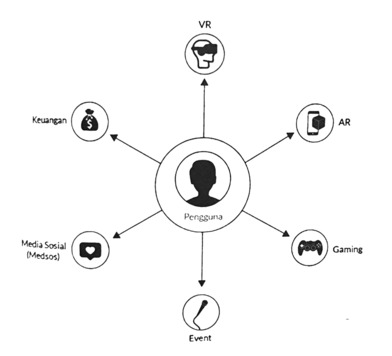
\includegraphics[scale=0.6]{gambar/img-metaverse-3.jpg}
  % Keterangan gambar yang diinputkan
  \caption{Metaverse tanpa \emph{blockchain}}
  % Label referensi dari gambar yang diinputkan
  \label{fig:Metaverse}
\end{figure}

% Contoh input gambar dengan format *.jpg
\begin{figure} [ht] \centering
  % Nama dari file gambar yang diinputkan
  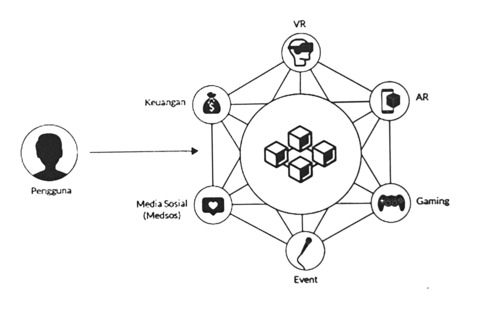
\includegraphics[scale=0.6]{gambar/img-metaverse-blockchain-4.jpg}
  % Keterangan gambar yang diinputkan
  \caption{Metaverse berbasis \emph{blockchain}}
  % Label referensi dari gambar yang diinputkan
  \label{fig:Metaverse Blockchain}
\end{figure}
